\section{Andere Anforderungen}
\section*{Anhang A: Glossar}
\label{glossar}
\begin{itemize}
\item Benutzer: Als Benutzer beschreiben wir einen Konsumenten des Softwareprodukts.
\item Support/Supporter: Als Supporter beschreiben wir eine angestellte Hilfsperson, mit eingeschränkten Berechtigungen, die dem Benutzer bei Problemen helfen kann.
\item Support Ticket: Ein Support Ticket ist ein Objekt welches die Kommunikation zwischen Supporter und Benutzer zu einem bestimmten Thema bündelt.
\item Admin: Der Admin ist eine angestellte Person, die Vollzugriff auf das gesamte System hat.
\item Externes Gerät: Das Externe Gerät, ist in der Lage automatisch Strom vom Stromzähler eines Benutzers einzulesen.
\item Immobilie: Immobilien sind in unserer Beschreibung Immobilien in denen der Benutzer seine Verbräuche erfassen möchte.
\item Verbrauchstyp: Der Verbrauchstyp ist die Art des Verbrauchs, zum Beispiel: Strom.
\item Einheit: Die Einheit beschreibt eine tatsächliche Einheit eines Verbrauchstyps, zum Beispiel: Kilowattstunde
\item Einseinheit: Die Einseinheit ist eine Einheit mit dem Umrechnungsfaktor 1. Diese muss für jeden Verbrauchstyp definiert sein.
\item Verbrauch: Der Verbrauch modelliert den tatsächlichen Wert des Verbrauchs in der Einseinheit über einen gewissen Zeitraum.
\item Zeitreihe: Eine Zeitreihe modelliert einen Verbrauch mit einem Verbrauchstyp.
\item Vergleichszeitreihe: Als Vergleichszeitreihen beschreiben wir Zeitreihen, die wir aus Nutzerdaten generieren oder aus externen Quellen erstellen. Diese dienen lediglich zum Vergleichen des Verbrauchs eines Benutzers.
\item Verbraucher: Ein Verbraucher ist ein Gerät einer Immobilie welches einen konstanten Verbrauch hat und somit automatisch täglich in eine Verbrauchszeitreihe eingetragen werden kann.
\end{itemize}
\section*{Anhang B: Modelle}
\subsection{Use-Case Diagramm}
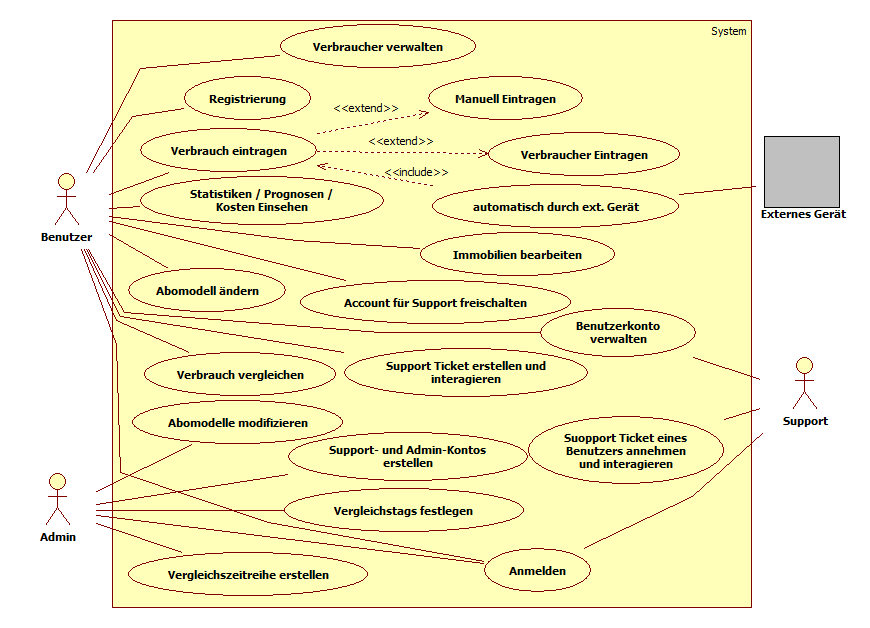
\includegraphics[scale=0.4]{use_case.png}

\subsection{Klassendiagramm}
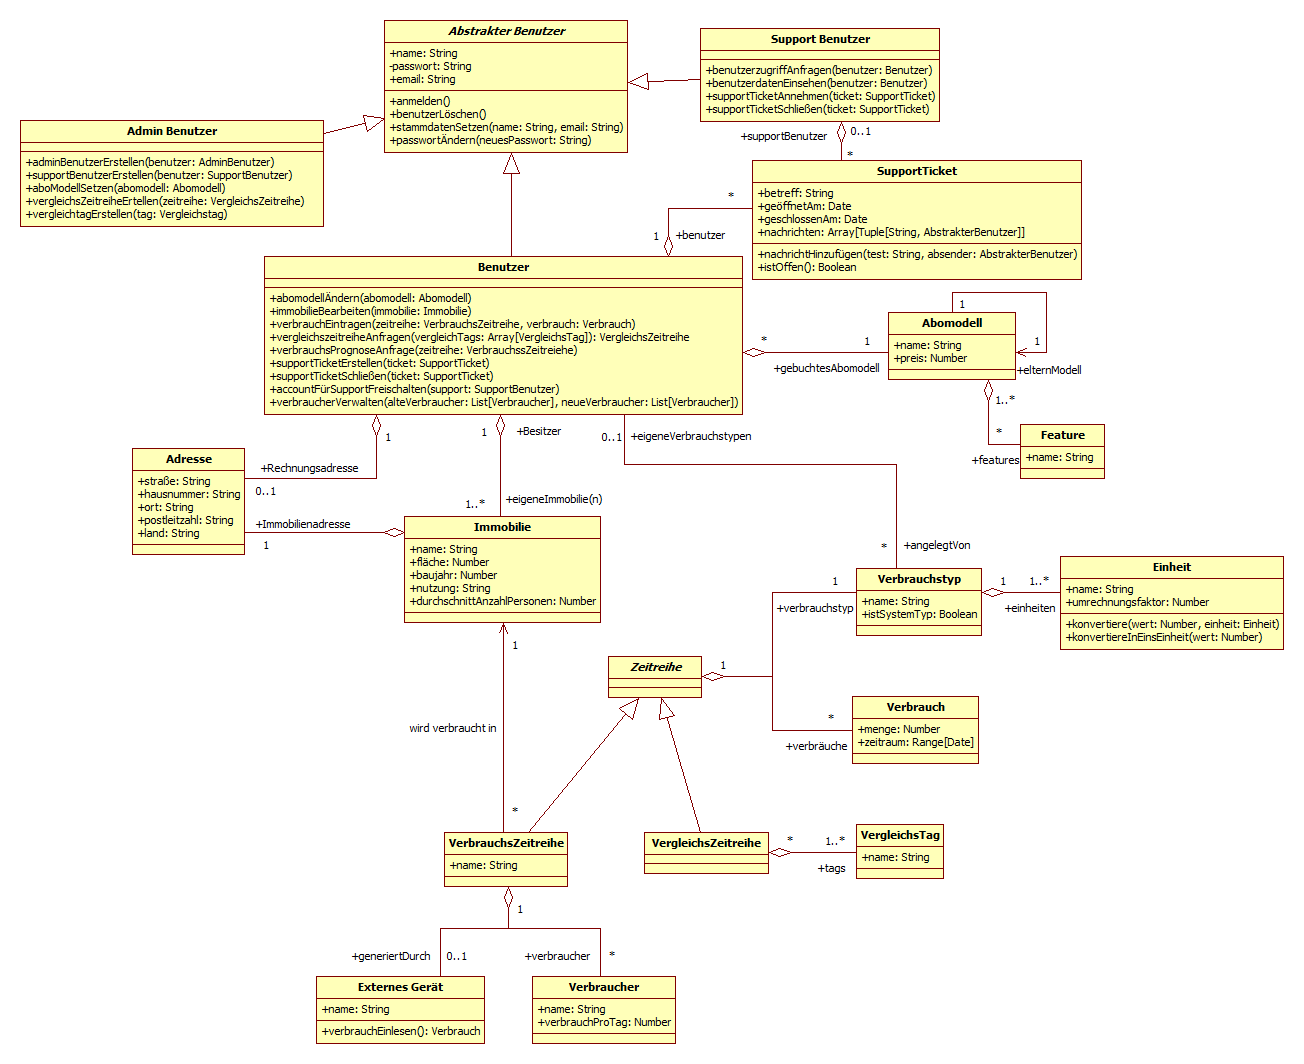
\includegraphics[scale=0.3]{klassendiagramm.png}

\section*{Anhang C: Offene Punkte}

\begin{itemize}
    \item Die Zuteilung der Features zu den Abomodellen.
    \item Die konkrete Wahl der unterstützten Zahlungsanbietern.
    \item Alle funktionalen Anforderungen die mit \gquote{Noch zu diskutieren} beschrieben sind.
    \item Die konkreten Anforderungen an die Schnittstelle für externe Geräte. 
\end{itemize}

